%-----------------------------------------------------------------------------%
\chapter{METODE PENELITIAN}
%-----------------------------------------------------------------------------%

%
\vspace{4.5pt}

\begin{flushleft}
   \section{Alur Penelitian}

   \section{Penjabaran Langkah Penelitian}
   \subsection{Langkah 1}

   \section{Alat dan Bahan Tugas Akhir}
   \subsection{Alat}
   \subsection{Bahan}
\end{flushleft}

\vspace{5cm}
\noindent \textbf{CONTOH Penulisan}
\section{Analisa Sistem}

\subsection{Analisa Sistem Saat Ini}
Analisa sistem pendukung keputusan dalam penentuan penjurusan dibuat oleh peneliti dalam bentuk use case diagram yang mewakili secara sederhana dan bisa dijadikan sebagai bahan dalam evaluasi sistem yang berjalan, sehingga sistem dapat terlihat tanpa harus mengetahui secara detail prosedur yang berjalan.
\begin{figure}[ht]
	\centering
	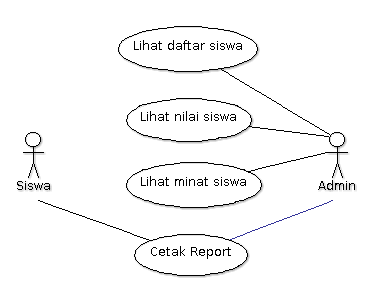
\includegraphics[width=10cm]{images/UseCaseDiagramSistemSaatIni}
	\caption{Use Case Diagram Analisa Sistem Saat Ini}
\end{figure}

\newpage
\noindent Dibawah ini merupakan deskripsi dari use case yang sedang berjalan:
\begin{enumerate}[nolistsep,leftmargin=0.5cm]
\item \textit{Admin} melihat daftar siswa.
\item \textit{Admin} melihat nilai setiap siswa.
\item \textit{Admin} melihat minat setiap siswa.
\item \textit{Admin} mencetak hasil keputusan.
\item Siswa melihat laporan penjurusan yang telah dicetak oleh \textit{admin}
\end{enumerate}

\subsection{Evaluasi Sistem Saat Ini}

\begin{table}[ht]
\centering
\caption{Permasalahan dan Solusinya}
\begin{tabular}{|>{\raggedright}p{5cm}|p{2.5cm}|>{\raggedright}p{5cm}|}
 \hline
 \multicolumn{1}{|c}{\bfseries Masalah} & \multicolumn{1}{|c|}{\bfseries Aktor} & \multicolumn{1}{c|}{\bfseries Solusi} \\ 
  \hline
\begin{enumerate}
   	\item Masalah masalah masalah Masalah masalah masalah Masalah masalah masalah Masalah masalah masalah.
   	\item Masalah masalah masalah Masalah masalah masalah Masalah masalah masalah Masalah masalah masalah.
   	\item Masalah masalah masalah Masalah masalah masalah Masalah masalah masalah Masalah masalah masalah.
   \end{enumerate} &
   \begin{enumerate}
  	\item Aktor 1
  	\item Aktor 2
  \end{enumerate} &
  \begin{enumerate}
  \item Solusi solusi solusi Solusi solusi solusi Solusi solusi solusi Solusi solusi solusi Solusi solusi solusi.
  \item Solusi solusi solusi Solusi solusi solusi Solusi solusi solusi Solusi solusi solusi Solusi solusi solusi.
  \item Solusi solusi solusi Solusi solusi solusi Solusi solusi solusi Solusi solusi solusi Solusi solusi solusi.
  \end{enumerate}
     \tabularnewline
  \hline
 \end{tabular}
\end{table}

\subsection{Model yang Diusulkan}

\subsection{Acitivity Diagram yang Diusulkan}

\subsection{Perancangan Prosedur Sistem}

\subsubsection{Use Case Diagram}

\subsubsection{Activity Diagram}
\begin{enumerate}[nolistsep,leftmargin=0.5cm]
\item \textit{Activity diagram} satu

\begin{enumerate}[label=\alph*.]
	\item Item 1.
	\item Item 2.
	\end{enumerate}
\item Dua
\end{enumerate}

\subsubsection{Class Diagram}

\subsubsection{Sequence Diagram}

\subsection{Perancangan Antarmuka (Interface)}

\newpage